

\section*{\hfil Questões e Respostas\hfil}



\section{Questão 3}
% Responda às perguntas seguintes com base no conteúdo da trama Ethernet que contém a mensagem de acesso ao servidor (HTTP GET encriptada).

\begin{figure}[H]
\centering
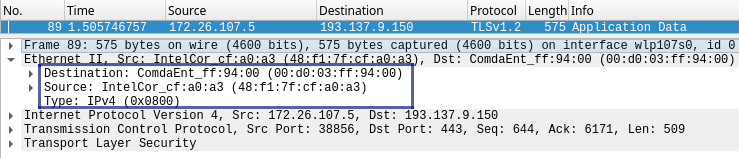
\includegraphics[width=500pt]{prints/Questao3/questao3.tramaClient.png}
\caption{Captura da Trama \textit{Ethernet} que contém mensagem de acesso.} \label{questao3-1}
\end{figure}


\subsubsection{Anote os endereços MAC de origem e de destino da trama capturada.}

    \par Estes endereços podem ser consultados no campo \textit{Source} e \textit{Destination}, respetivamente, no cabeçalho da trama \textit{Ethernet}, tal como se demonstra com a Figura \ref{questao3-1}:

    \begin{multicols}{2}
    \begin{itemize}
        \item MAC Origem: \textbf{48:f1:7f:cf:a0:a3}  
        \item MAC Destino: \textbf{00:d0:03:ff:94:00}
    \end{itemize}
    \end{multicols}
    




\paragraph{}
\subsubsection{Identifique a que sistemas se referem. Justifique.}

    \par O endereço MAC de origem refere-se à máquina nativa utilizada nesta questão, tendo esta o endereço IP 172.26.107.5. No caso do endereço MAC destino, este refere-se ao sistema destino do próximo salto na rede, isto é, ao \textit{router} de acesso ou \textit{default gateway}, uma vez que, contrariamente ao nível de rede (protocolo IP), o nível de ligação lógica vai recalculando \textbf{salto-a-salto} o endereço MAC destino contido na trama até chegar ao endereço coincidente com o endereço IP destino, neste caso, 193.137.9.150.




\paragraph{}
\subsubsection{Qual o valor hexadecimal do campo \textit{Type} da trama \textit{Ethernet}? O que significa?}

    \par O campo \textit{Type} tem como valor \textbf{0x0800}, que representa o protocolo \textit{IPv4}, ou seja, este campo indica qual o protocolo que está a ser encapsulado pela trama.




\subsubsection{Quantos \textit{bytes} são usados no encapsulamento protocolar, i.e. desde o início da trama até ao início dos dados do nível aplicacional (Application Data Protocol: http-over-tls)? Calcule e indique, em percentagem, a sobrecarga (\textit{overhead})
introduzida pela pilha protocolar}

    \begin{figure}[H]
    \centering
    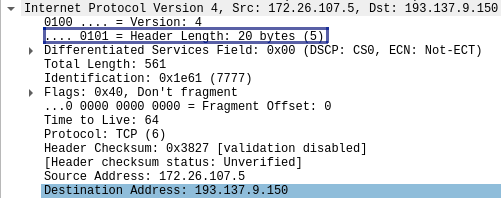
\includegraphics[width=280pt]{prints/Questao3/questao3-IP.png}
    \caption{Protocolo IP encapsulado.} \label{questao3-d-IP}
    \end{figure}
    
    \begin{figure}[H]
    \centering
    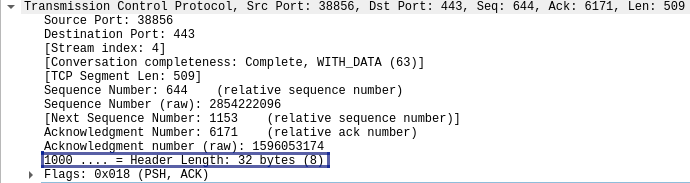
\includegraphics[width=380pt]{prints/Questao3/questao3-TCP.png}
    \caption{Protocolo TCP encapsulado.} \label{questao3-d-TCP}
    \end{figure}
    
    \paragraph{}
    \par Neste caso são vários os protocolos encapsulados pela trama \textit{Ethernet}, como, por exemplo, o protocolo IP (nível de rede) e TCP (nível de transporte). Assim, conseguimos somar o tamanho de todos os cabeçalhos (\textit{Ethernet}, IP, TCP) utilizados para encapsular os dados do nível aplicacional (\textit{Application Data Protocol}), obtendo o seguinte resultado: 
    
    \begin{align*}
        {14 \:(\textit{Ethernet}) + 20 \:(IP) + 32 \:(TCP) = \textbf{66}\:\textit{bytes}}
    \end{align*} 

    
    
    \par Pelos cálculos, obtivemos um total de 66 \textit{bytes} de encapsulamento protocolar. Relativamente à \textbf{sobrecarga} (\textit{overhead}), esta terá o valor de: 
    
    \begin{align*}  
        \frac{66\:(\textit{headers})}{575\:(tamanho\:total)*} = \textbf{11,5}\:\%  
    \end{align*}  
    
    
    \par \textbf{* NOTA:} O tamanho total da trama com a inclusão dos cabeçalhos foi verificada na Figura \ref{questao3-1} na primeira linha referente à informação do \textit{Frame}.  






% A seguir responda às seguintes perguntas, baseado no conteúdo da trama Ethernet que contém o primeiro byte da resposta HTTP proveniente do servidor
\subsubsection{Qual é o endereço \textit{Ethernet} da fonte? A que sistema de rede corresponde? Justifique.}

    \begin{figure}[H]
    \centering
    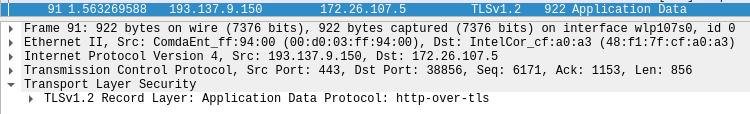
\includegraphics[width=500pt]{prints/Questao3/questao3-respostaServer.png}
    \caption{Captura da Trama \textit{Ethernet} de resposta.} \label{questao3-resposta1}
    \end{figure}


    \par O endereço \textit{Ethernet} da fonte é \textbf{00:d0:03:94:00} que corresponde ao sistema que na trama capturada nas alíneas anteriores estava no endereço MAC destino, ou seja, o \textit{router} de acesso ou \textit{default gateway} (último salto na rede até à máquina nativa).





\subsubsection{Qual é o endereço MAC do destino? A que sistema corresponde?}

    \par O endereço MAC destino é \textbf{48:f1:7f:cf:a0:a3} e corresponde à máquina nativa utilizada para responder a esta questão. Podemos confirmar pela análise à trama utilizada nas alíneas anteriores, pois este endereço corresponde ao endereço MAC origem da mesma.




\subsubsection{Atendendo ao conceito de desencapsulamento protocolar, identifique os vários protocolos contidos na trama recebida.}

    \paragraph{}
    \par Segundo o modelo OSI, existem sete camadas protocolares, onde podemos denotar a independência e modularidade entre as mesmas. Isto é, cada camada é desenvolvida de forma independente das outras, tendo responsabilidades e funcionalidades distintas, fornecendo serviços à camada diretamente acima e utilizando serviços da camada diretamente abaixo.
    
    \par Assim, cada nível protocolar utiliza uma PDU (\textit{Protocol Data Unit}) única com informações pertinentes que apenas consegue ser interpretada e manipulada pelas camadas homólogas. Desta forma, quando uma camada utiliza os serviços da camada de baixo, a informação que é transportada para o nível inferior vai ser encapsulada pelo mesmo, ou seja, por exemplo, a camada A envia os seus dados para a camada B (nível inferior) em formato \textit{PDU-A}, que, por sua vez, são encapsulados pela camanda B para \textit{PDU-B}.
    
    \par Em consequência, conforme os dados vão sendo enviados para as camadas inferiores, existe um encapsulamento protocolar sucessivo até ser atingido o nível mais baixo. Como tal, no caso em estudo, podemos denotar os vários protocolos encapsulados:

    
    \begin{figure}[H]
    \centering
    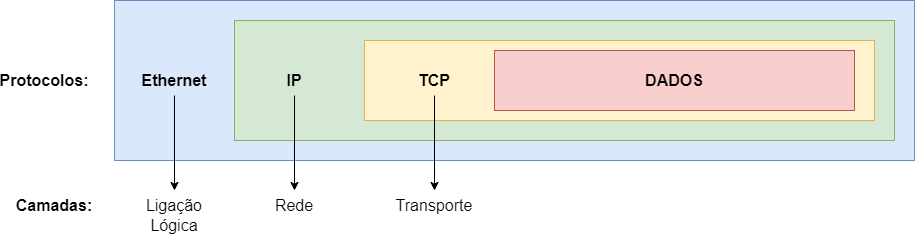
\includegraphics[width=450pt]{prints/Questao3/encapsulamento.png}
    \label{questao3-resposta2}
    \end{figure}

